\begin{frame}{La producción de información científica}
	\centering
	\only<1>{
		\framesubtitle{¿Por qué es los científicos necesitan nuevos sensores?}
		\begin{tikzpicture}
			\node(gerschman) {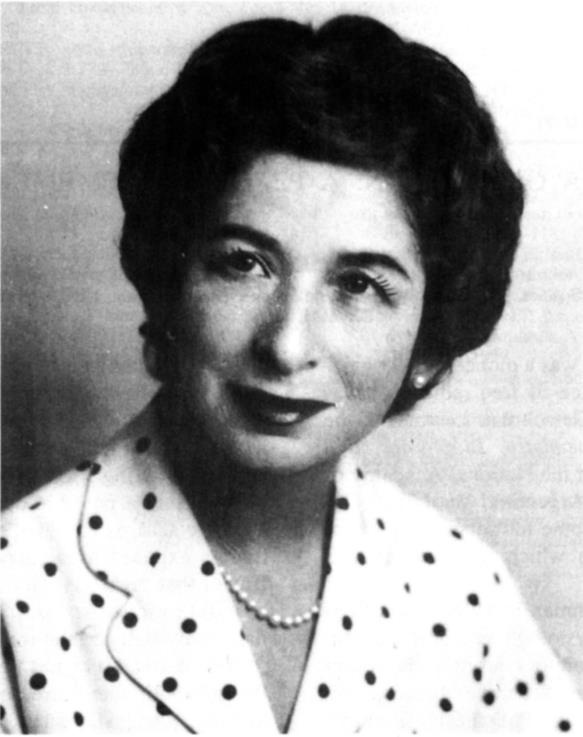
\includegraphics[width=.1\textwidth]{gerschman.jpg}};
		\end{tikzpicture}
		\huge{¿Qué es la Ciencia?}
		}
	\only<2>{
		\framesubtitle{otro subtitulo}
		}

\end{frame}
\begin{frame}{La producción de información científica}
	\begin{itemize}
		\item Los avances en las escalas de integración de circuitos permiten desarrollar sensores que recolectan mayor volumen de datos.
		\item Los nuevos sensores necesitan nuevos circuitos adicionales que les permitan adquirir datos y controlar su funcionamiento.
		\item El empleo de FPGA es muy útil para sintetizar circuitos digitales de alta velocidad.
		\item Los datos deben ser procesados para transformase en información.
		\item Los datos se deben transmitir desde los sistemas generadores a los sistemas procesadores.
	\end{itemize}
\end{frame}
%ACA me gustaría poner un frame donde se explique en forma gráfica lo de los sitemas procesadores y sistemas generadores
\begin{frame}{La necesidad de una comunicación\\entre un FPGA y una PC}
	\begin{itemize}
		\item Las computadoras son herramientas muy útiles para procesar datos.
		\item Los FGPA pueden operar a altas velocidades y realizar procesos en paralelo.
		\item Es de utilidad una comunicación entre las PC y las aplicaciones que utilizan FPGA para la implementación de circuitos.
		\item USB es una opción robusta, con ancho de banda suficiente para transmitir imágenes e incorporada en cualquier PC moderna.
	\end{itemize}
\end{frame}